\subsection{Beispiele}
    
    \subsubsection{Spannungswaage}
        Kräftegleichgewicht\\
        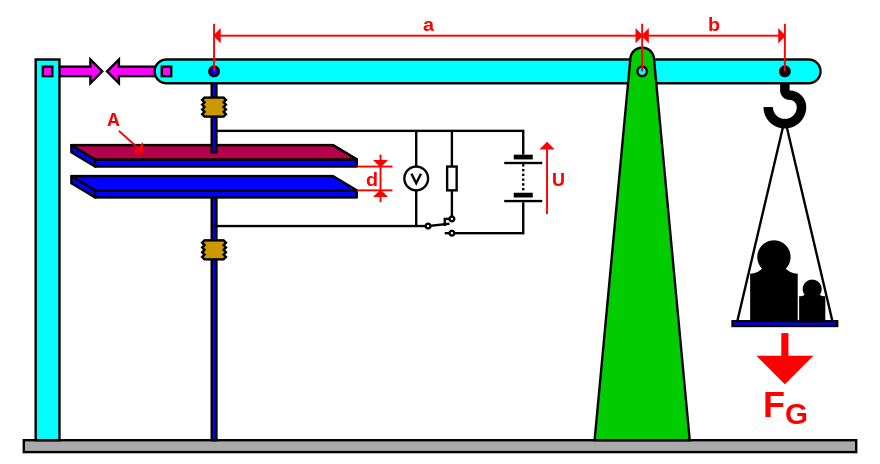
\includegraphics[width = 0.99\linewidth]{src/images/spannungswaage.png}
        \begin{minipage}{0.63\linewidth}
            \begin{empheq}[box = \fbox]{align*}
                F_E &= \frac{E \cdot Q}{2} = \frac{1}{2} \varepsilon_0 \varepsilon_r \frac{A}{d^2} U^2\\
                F_G &= m \cdot g\\
                a \cdot F_E &= b \cdot F_G
            \end{empheq}
        \end{minipage}
        \begin{minipage}{0.35\linewidth}
            \begin{scriptsize}
                \begin{empheq}{align*}
                    F_E &= \text{elektrostatische Kraft}\\
                    F_G &= \text{Gewichtskraft}\\
                    m &= \text{Masse} [kg]\\
                    g &= \text{Fallbeschleunigung}\\
                    E &= \text{Elektrische Feldstärke}\\
                    Q &= \text{Ladungsmenge}\\
                    \varepsilon_r &= \text{Permittivität}
                \end{empheq}
            \end{scriptsize}
        \end{minipage}